\subsection{Quantizzazione}
La quantizzazione piò essere vista come l'operazione "gemella" del campionamento in quanto si occupa di discretizzare i valori
del segnale ad ogni istante/campione $t$. Anticipiamo già che questa operazione fa perdere irreversibilmente dei bit di informazione
per cui è impossibile ricostruire esattamente il segnale di partenza dopo averlo quantizzato.\\
Consideriamo ora un segnale con un limitato $x_{\text{min}}\leq x(t) \leq x_\text{MAX}$. Discretizziamo l'intervallo $\left[x_{\text{min}}; x_\text{MAX}\right]$ in
un numero M di intervalli $I = 0,1,\dots,M-1$. Definiamo ora \textbf{soglia} $t_i$ l'estremo di un intervallo, t.c.:
\begin{equation*}
    I_i = [t_i;t_{i+1}]
\end{equation*}
Inoltre $t_0 = x_\text{min}$ e $t_M = x_\text{MAX}$
La quantizzazione consiste nel \textbf{sostituire} un valore $x \in I_i$ con il valore rappresentativo dell'intervallo $I_i$ detto $x_i$
Tutti i valori rappresentativi determinano \textbf{il dizionario di quantizzazione } $Q = \{x_0,x_1,\dots,x_{M-1}\}$.
Nella nostra trattazione, la quantizzazione che studieremo è \textbf{uniforme} ossia:
\begin{itemize}
    \item Tutti gli intervalli hanno uguale ampiezza $\Delta$ detto \textbf{passo di quantizzazione}:
    \begin{equation}
        \Delta = \frac{x_\text{MAX} - x_\text{min}}{M}
    \end{equation}
    \item Il valore rappresentativo $x_i$ è il valor medio:
    \begin{equation}
        x_i = \frac{t_i + t_{i + 1}}{2}
    \end{equation}
\end{itemize}
\newpage
\paragraph{Grafico di Quantizzazione.}Possiamo rappresentare un grafico che aiuta a capire il grado di approssimazione,
e dunque l'errrore, della quantizzazione sul segnale:\\
\begin{tikzpicture}[scale=1.2]

    % Assi
    \draw[->] (-5,0) -- (5,0) node[below] {$x$ (ingresso continuo)};
    \draw[->] (0,-5) -- (0,5) node[left] {$Q(x)$ (valore quantizzato)};
    
    % Linee di quantizzazione
    \foreach \k in {-4,-3,...,3} {
        % Calcolo del centro (valore rappresentativo)
        \pgfmathsetmacro{\center}{\k + 0.5};
        
        % Disegno del livello quantizzato (scalini)
        \draw[thick,red,smooth] plot[domain=\k:\k+1,samples=2] (\x,{\center});
        
        % Punti centrali rappresentativi
        \filldraw (\k+0.5,{\center}) circle (1.5pt) node[right] {};
    }
    
    % Linee guida verticali
    \foreach \k in {-4,-3,...,4} {
        \draw[thick,blue,dashed] (\k,-4) -- (\k,4); % Linee guida
    }
    
    % Annotazioni intervalli
    \foreach \k in {-4,-3,...,3} {
        \pgfmathsetmacro{\center}{\k + 0.5};
        \draw[dashed] (\k+0.5,0) -- (\k+0.5,{\center});
        \node[below] at (\k+0.5,0) {$x_{k}$};
    }
    
    % Linea guida ideale
    \draw[thick,dashed,gray] (-4,-4) -- (4,4) node[above] {$y = x$ (valore continuo)};
    
    % Etichette
    \node at (-2.5,1.5) [align=center,red] {Livelli \\ rappresentativi \\ (medie)};
    \node[below right] at (1,0.5) {$\Delta$};
    
    \end{tikzpicture}

Possiamo descrivere dunque la quantizzazione come un sistema $x_q(t) = Q[x(t)] = x_i$ con $x_t \in I_i$.Da tutto ciò possiamo
notare alcune cose:
\begin{itemize}
    \item La quantizzazione è una relazione 1-a-molti (un valore rappresentativo a infiniti valori dell'intervallo)
    \item La quantizzazione introduce un errore $e_q = x_q - x$
\end{itemize}
Per questi motivi, quest'operazione danneggia irreversibilmente la qualità del suono.

\subsubsection{Errore di Quantizzazione}
Dell'errore di quantizzazione possiamo innanzitutto dire che $-\frac{\Delta}{2} \leq e_q \leq \frac{\Delta}{2}$ con $\Delta = \frac{x_\text{MAX} - x_\text{min}}{2} $.
Inoltre, dal momento che dovremo lavorare nel mondo digitale, per agevolare la rappresentazione in bit del valore quantizzato si usa
un $M = 2^n$, questa viene detta \textbf{quantizzazione su n bit}.
Si può dimostrare che per intervalli sufficientemente piccoli, l'errore di quantizzazione ha distribuzione \textbf{uniforme discreta}, ossia 
ha una funzione di densita di probabilità $f_{e_q} = \frac{1}{\Delta}$. Consideriamo ora che possiamo riscrivere un valore rappresentativo nella seguente forma:
\begin{equation}
    x_q(t) = x(t) + e_q(t)
\end{equation}
Quindi possiamo vedere $e_q(t)$ come un vero segnale e possiamo analizzarlo nel dominio delle frequenze. Dunque possiamo osservare ora che:
\begin{itemize}
    \item Dal momento che $-\frac{\Delta}{2} \leq e_q \leq \frac{\Delta}{2}$ (con $\Delta \gg 1$) allora la potenza di $e_q$ sarà molto minore della potenza di $x(t)$
    \item Dal grafico che il professore ha reso disponibile sul suo sito emerge che $e_q$ è molto "nervoso", ossia cambia repentinamente valore in intorni abbastanza piccoli,
    per questo motivo possiamo intuire che, nel dominio delle frequenze, questo errore sarà composto da frequenze molto alte e quindi avrà una banda MOLTO AMPIA.
\end{itemize}

Provando ad applicare un filtro passa-basso al segnale $X(f)$ e all'errore $E_q(f)$ otteniamo che, nel filtro, l'errore si ripiegherà 
su se stesso più volte (tante volte) fino ad esaurirsi. Possiamo accorgerci che la somma di tutti questi ripiegamenti è costante, dunque
possiamo rappresentare la situazione nel dominio delle frequenze nella seguente maniera, cioè $X_R(f) = X(f)E_{q_r}(f)$:\\
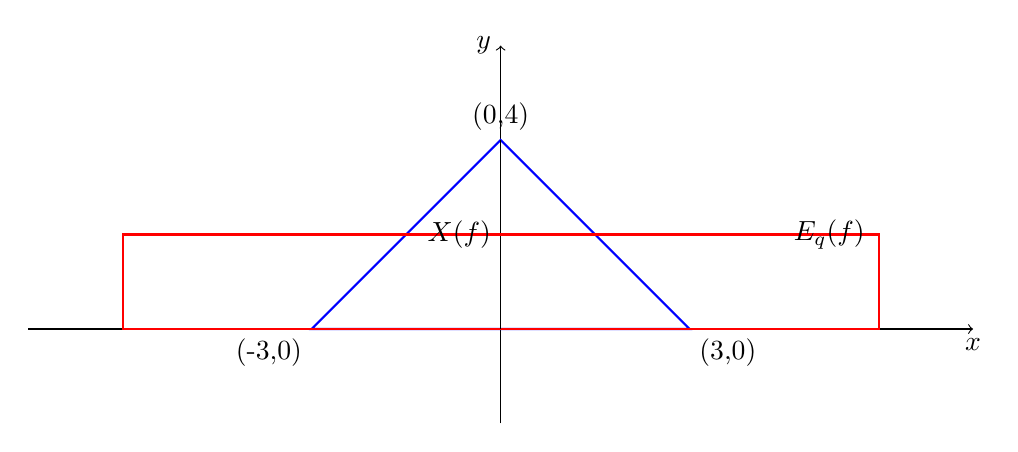
\begin{tikzpicture}[scale=1.2]

    % Assi
    \draw[->] (-5,0) -- (5,0) node[below] {$x$};
    \draw[->] (0,-1) -- (0,3) node[left] {$y$};
    
    % Vertici del triangolo
    \coordinate (A) at (-2,0); % Sinistra
    \coordinate (B) at (2,0);  % Destra
    \coordinate (C) at (0,2);  % Vertice superiore
    
    % Disegno del triangolo
    \draw[thick,blue] (A) -- (B) -- (C) -- cycle;
    
    % Rettangolo che condivide la base
    \draw[thick,red] (-4,0) rectangle (4,1);
    
    % Annotazioni
    \node[below left] at (A) {(-3,0)};
    \node[below right] at (B) {(3,0)};
    \node[above] at (C) {(0,4)};
    \node[right] at (3,1) {$E_q(f)$};
    
    % Tratteggio verticale per evidenziare l'altezza
    \draw[dashed] (0,0) -- (0,2) node[midway,left] {$X(f)$};
    
    \end{tikzpicture}

Possiamo dunque vedere $e_q(t)$ come un vero e proprio \textbf{rumore bianco} i cui contributi di ogni frequenza sono costanti